\documentclass[10pt,a4paper]{article}
\usepackage[margin=22mm]{geometry}\usepackage[T1]{fontenc}\usepackage{lmodern,microtype,booktabs,graphicx,xcolor,hyperref,tcolorbox,parskip}
\definecolor{ink}{HTML}{172B4D}\definecolor{teal}{HTML}{176B87}\definecolor{coral}{HTML}{D06A45}\definecolor{mist}{HTML}{F1F6F8}
\hypersetup{colorlinks=true,linkcolor=teal,urlcolor=teal}
\title{\vspace{-2em}\color{ink}\bfseries IDM-Viz selective-label bias audit\\[-.2em]\large Feature-targeted labels with a known-probability random audit}
\author{Phase 3 controlled synthetic addendum}\date{17 November 2026}
\begin{document}\maketitle\vspace{-1em}
\begin{tcolorbox}[colback=mist,colframe=teal,boxrule=0pt,leftrule=2mm]\textbf{Scope.} Simulated acquisition on two synthetic families and two conditions. This is not a prospective natural-stream label audit.
\end{tcolorbox}
\section*{Protocol}
We evaluated 30 fixed seeds, linear and five-region generators, stationary and abrupt conditional reversal, and 96 consecutive batches of 500 rows. Acquisition sees only the frozen classifier's confidence, never labels. A targeted-only policy selects exactly the 10\% least-confident rows; its inclusion probability is zero outside that set, so population accuracy is not identifiable from these labels and no IPW estimate is reported. The combined policy includes that certainty sample and Bernoulli-samples each remaining row with probability 0.10 (logged \(\pi_i=1\) or \(0.10\)). A simple random audit with probability 0.19 matches the combined policy's expected 19\% label budget. We compute the untruncated Horvitz--Thompson accuracy \(N^{-1}\sum_{i\in S} c_i/\pi_i\) and its Bernoulli design variance. Inference summaries average batches within seed and bootstrap the 30 seeds (5000{} replicates). Batch-level normal intervals are also checked against fully available synthetic truth, used only after selection for evaluation.
\section*{Findings}
For linear conditional reversal, the evaluator's mean full-stream accuracy was 0.388{} (95\% seed-bootstrap CI 0.387{}--0.388{}). The targeted-only selected-label estimate was 0.487{} (0.485{}--0.489{}), showing that the direction and size of selection bias depend on the stream. With the random-audit component, the naive selected-label estimate was 0.435{} (0.433{}--0.437{}), while the logged-probability Horvitz--Thompson estimate was 0.388{} (0.385{}--0.390{}). The budget-matched simple-random Horvitz--Thompson estimate was 0.387{} (0.385{}--0.389{}). The combined policy sampled a mean of 95.0{} labels per 500-row batch. Its normal design interval covered the finite-batch truth in 0.934{} of batch-seed cases. This empirical coverage is below or near nominal and is not a guarantee.
\begin{center}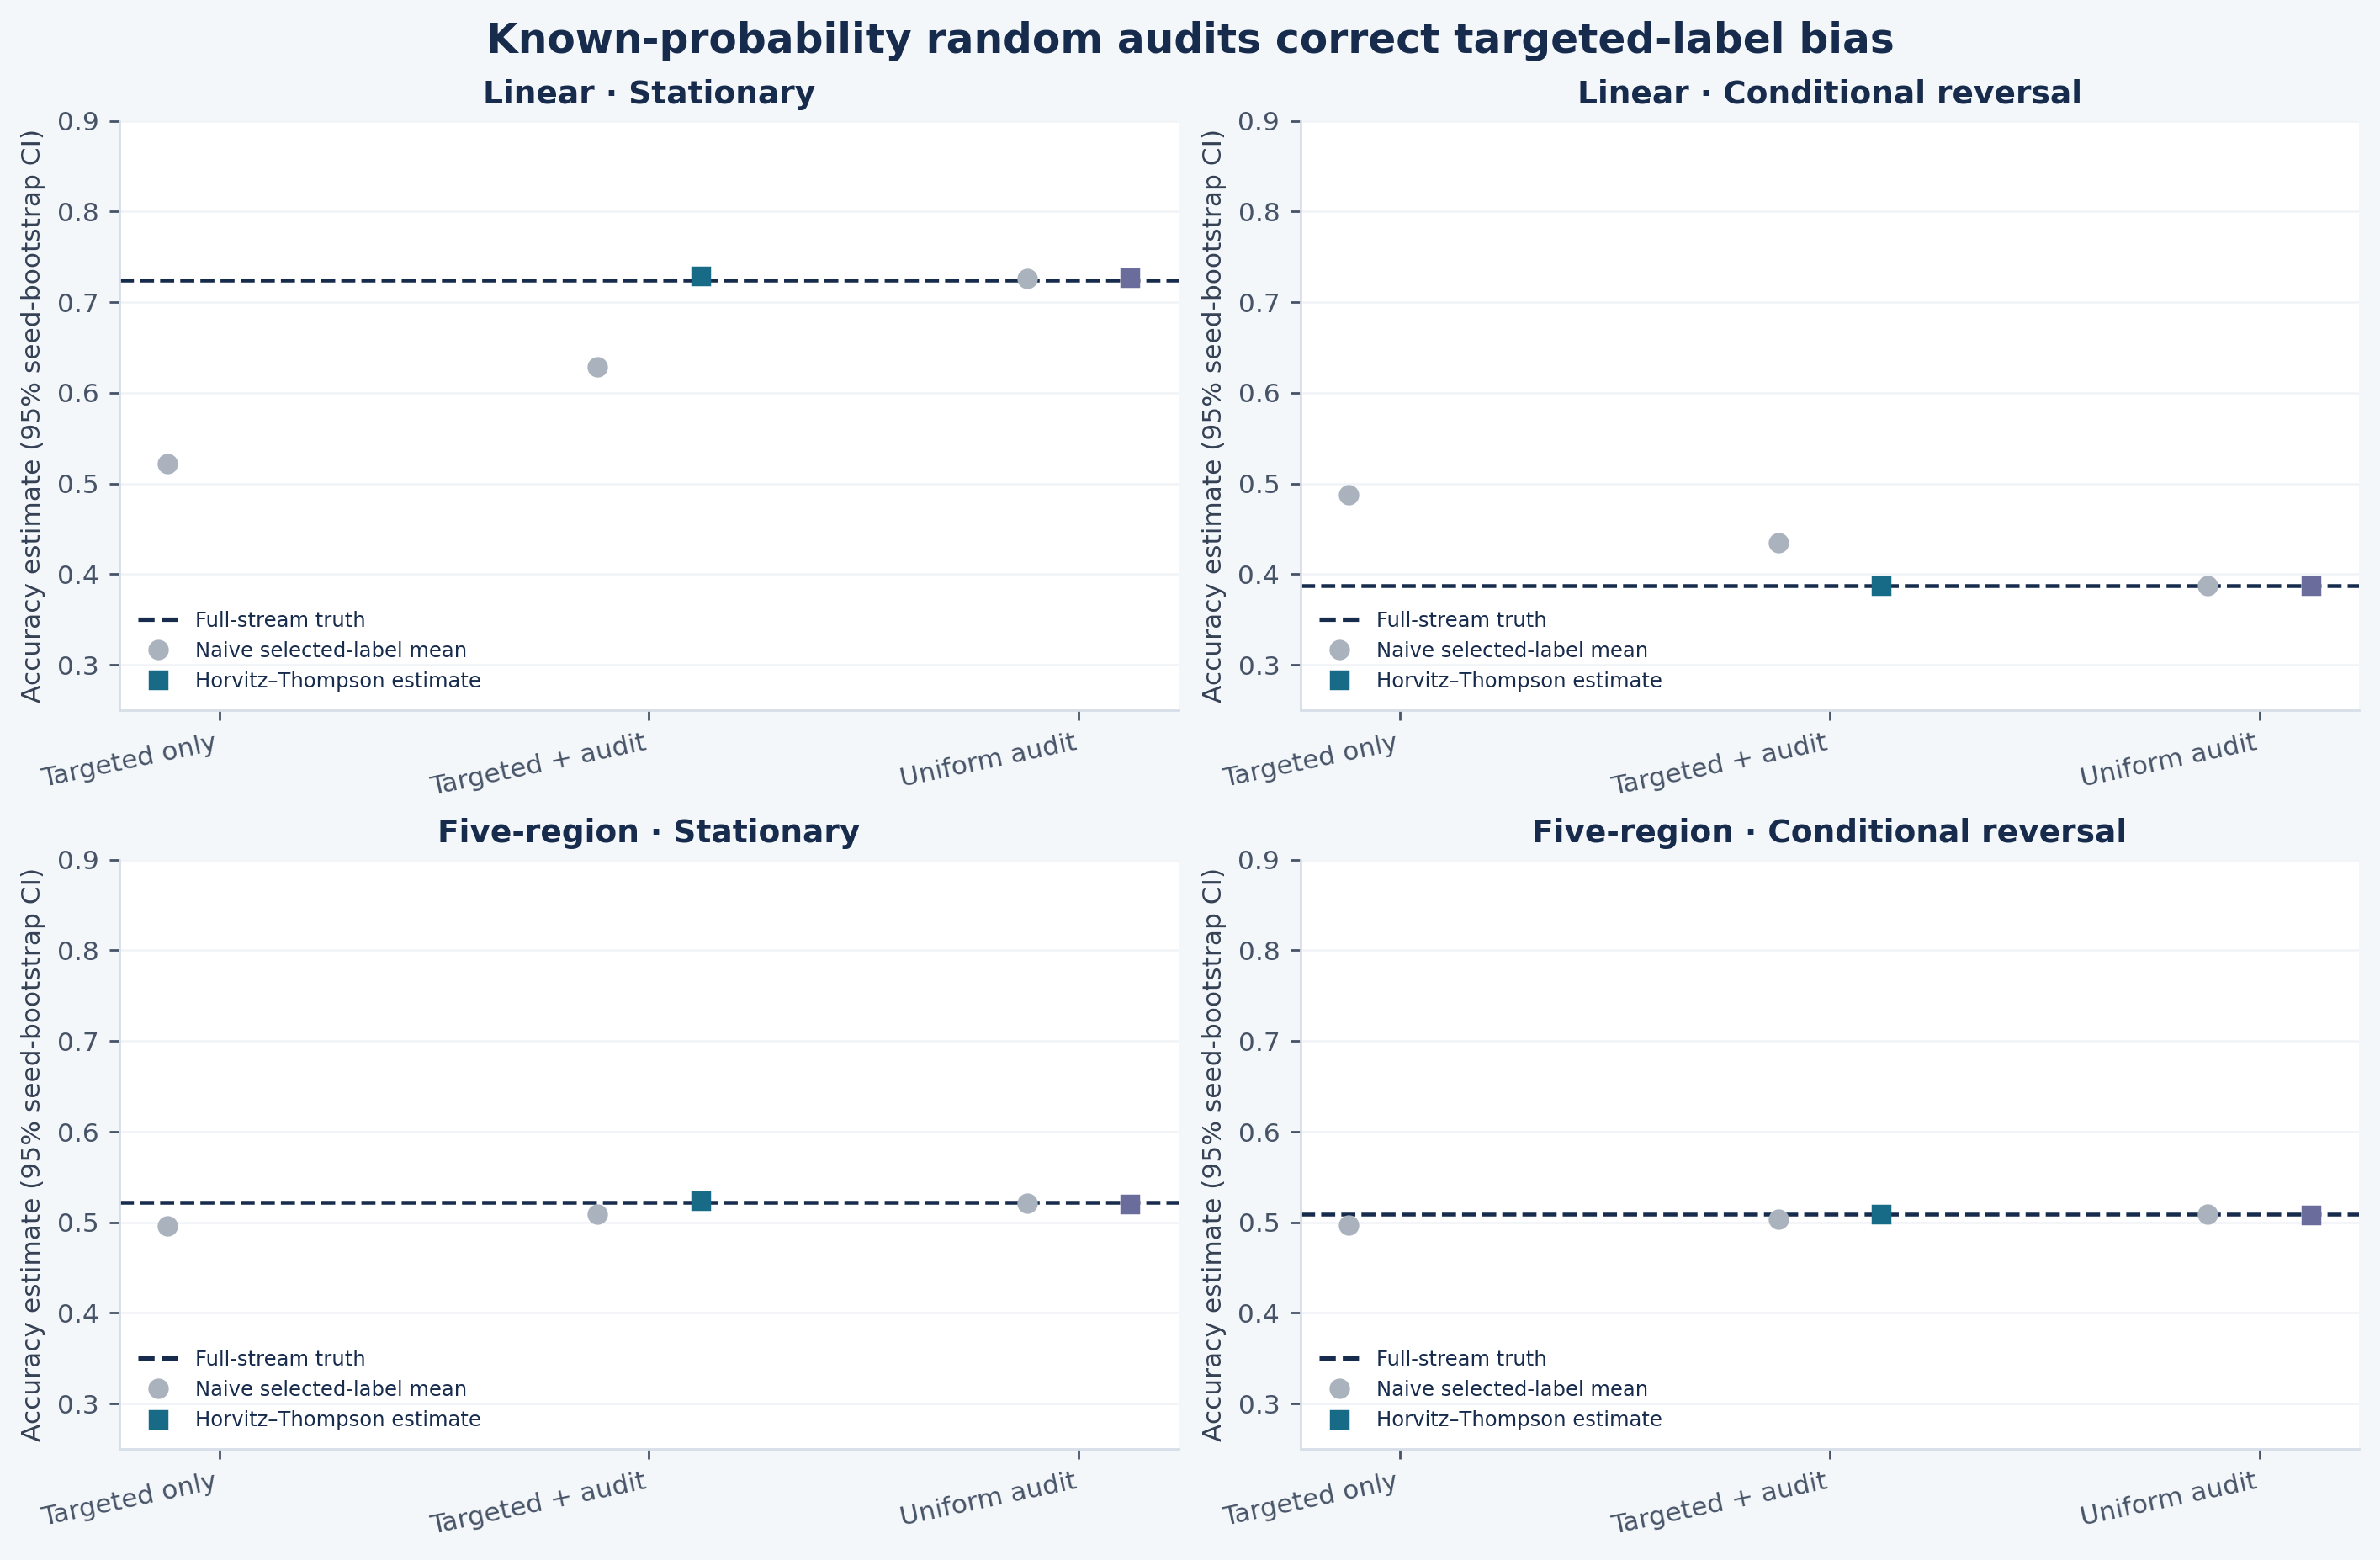
\includegraphics[width=\linewidth]{selective_label_bias.png}\end{center}
\section*{Interpretation and limits}
Targeted labels can efficiently find errors but their unweighted mean does not estimate population accuracy. A known-probability random component restores positivity and permits design-based weighting in this simulated setting; it does not make the deterministic targeted-only sample representative. Horvitz--Thompson estimates and normal intervals are intentionally not clipped to \([0,1]\). Only these synthetic selection laws, inclusion probabilities, fixed classifier, and batch sizes are evaluated. Natural acquisition behavior, label costs, nonresponse, misspecified probabilities, and calibration refits from selected outcomes remain untested. The logged outcomes contain only selected rows; all unseen truth is used solely for evaluator scoring.
\section*{Reproduction}
Run \texttt{python scripts/run\_selective\_label\_audit.py} then \texttt{python scripts/summarize\_selective\_label\_audit.py}. Full selected-label inclusion probabilities, batch estimates, seed-bootstrap summaries, source hashes and the editable TeX source are included.
\end{document}
